\subsection{Homogeneity}

Recall that a function $h: \R^n \to N$ is homogeneous of degree zero at $y \in \R^n$ if it is radially-invariant about $y$, i.e. for every $\lambda > 0$ and $x \in \R^n$ we have
	\[ h(y + x) = h(y + \lambda x). \]
We say that $h$ is \emph{$k$-homogeneous} if it translation-invariant in the directions spanned by a $k$-plane $V^k \subseteq \R^n$, i.e. for every $x \in \R^n$ and $v \in V^k$, we have
	\[ h(x) = h(x + v). \]
\begin{remark}
	A function is $k$-homogeneous if and only if depends on $(n - k)$-variables and is radially-invariant. This furnishes the bijective correspondence 
		\[\{ \text{$k$-homogeneous maps $h: \R^n \to N$} \}\leftrightarrow \{ \text{maps $h: S^{n - k - 1} \to N$}\} \times \{ \text{$k$-planes $V^k \subseteq \R^n$} \} \times \{ \text{centers $y \in \R^n$} \}. \]
	The space of $k$-planes is known as the \textit{Grassmannian}, and there is a natural choice of smooth structure such that it forms a compact manifold. Thus if we consider $L^2$-maps, a bounded sequence will admit a subsequence converging weakly to another $k$-homogeneous map.  	
\end{remark}	
	

For $f : B_r (y) \to N$, define the \emph{deviation} from a $k$-homogeneous map about $y \in \R^n$ at scale $r > 0$ by  
	\[ \sfD^{k} (f, B_r (y)) := \inf_h \frac{1}{|B_r (y)|} \int_{B_r (y)} |f - h|^2 \, \dV , \]
where $h : \R^n \to N$ are taken over $k$-homogeneous maps. Note that the deviation is scale invariant. Furthermore, we see that the infimum is actually achieved from weak compactness of a minimising sequence and weak lower-semicontinuity of the integral. We say that $f$ is \emph{$(\epsilon, r, k)$-homogeneous} at $y \in \R^n$ if $\sfD^k (f, B_r (y)) < \epsilon$. 

\subsection{Rigidity}

For a stationary harmonic map $f: B_2 (0) \to N$, we know that it satisfies the monotonicity formula
	\[ \theta_r (y) - \theta_s (y) = \int_s^r \int_{\partial B_\rho (y)} \frac{1}{\rho^{n - 2}} \left| \frac{\partial f}{\partial \rho} \right|^2 d\rho \dA. \]	
It follows that $\theta_s (y) = \theta_r (y)$ if and only if $f$ is radially-invariant about $y$ on the annulus $s < |x - y| < r$. We can upgrade this qualitative rigidity statement to a quantitative rigidity statement concerning homogeneity via a contradiction argument. 

\begin{lemma}[Quantitative rigidity]
	Let $f: B_2 (0) \to N^m$ be a stationary harmonic map with bounded energy $E[f] \leq \Lambda$. For every $\epsilon > 0$, there exists $\delta, r \ll_{n, N, \Lambda, \epsilon} 1$ such that if
		\[ \theta_1 (0) - \theta_r (0) \leq \delta, \]
	then $f$ is $(\epsilon, 1, 0)$-homogeneous at $0$. 	\label{lem:rigid}
\end{lemma}

\begin{proof}
	Assume otherwise for some $\epsilon > 0$, then there exists a sequence of stationary harmonic maps $f_i : B_2^n (0) \to N$ with bounded energy $E[f_i] \leq \Lambda$ such that 
		\[ \theta_1 [f_i] (0) - \theta_{1/i} [f_i] (0) \leq \frac1i,\]
	however $f_i$ are not $(\epsilon, 1, 0)$-homogeneous. By weak compactness of $H^1 (B_2^n (0); N)$ and also its compact embedding into $L^2 (B_2^n (0); N)$, we may pass to a subsequence $\{ f_{i_k} \}_k$ converging to $f : B_2^n (0) \to N$ weakly in $H^1 (B_2^n (0); N)$ and strongly in $L^2 (B_2^n (0); N)$. From weak convergence and the monotonicity formula, 
		\begin{align*}
			 0 
			 	&= \lim_{k \to \infty} \theta_1 [f_{i_k}] (0) - \theta_{1/i} [f_{i_k}] (0) \\
			 	&= \lim_{k \to \infty} \int_{1/i_k}^1 \int_{\partial B_\rho (0)} \frac{1}{\rho^{n - 2}} \left| \frac{\partial f_{i_k}}{\partial \rho} \right|^2 d\rho \dA = \int_{0}^1 \int_{\partial B_\rho (0)} \frac{1}{\rho^{n - 2}} \left| \frac{\partial f}{\partial \rho} \right|^2 d\rho \dA
		\end{align*}	 
	which implies $\partial_\rho f \equiv 0$, i.e. $f$ can be extended radially to a $0$-homogeneous map on $\R^n$. However by strong convergence,
		\[ \sfD (f_{i_k}, B^n_1 (0)) \leq  \frac{1}{|B_1^n (0)|} \int_{B_1 ^n(0) }  |f_{i_k} - f|^2 \, \dV \overset{k \to \infty}{\longrightarrow} 0, \]
	which implies $f_{i_k}$ are $(\epsilon, 1, 0)$-homogeneous for $k \gg 1$, a contradiction. 
\end{proof}

\subsection{Cone-splitting}


The cone-splitting principle allows us to upgrade our symmetries provided linear independence. That is, if a measurable map $f: \R^n \to N$ is 
	\begin{enumerate}
		\item $k$-homogeneous at $0$ with respect to a plane $V^k \subseteq \R^n$, and
		\item $0$-homogeneous at $y \not\in V^k$,
	\end{enumerate}
then $f$ is	$(k + 1)$-homogeneous at $0$ with respect to the $(k+ 1)$-plane $\operatorname{span} \{ y, V^k \}$.

\begin{example}
	Denote $x' := (x_1, x_2)$, consider $f: \R^3 \to \R$ given by $f (x) := x'/|x'|$. Observe that $f$ is $0$-homogeneous at $(0, 0, 0)$ and $(0, 0, 1)$, hence it is $1$-homogeneous at $0$ with respect to the $x_3$-axis.
\end{example}

The quantitative version follows an analogous contradiction argument as in the proof of quantitative rigidity.

\begin{lemma}[Quantitative cone-splitting]
	Let $f: B_2 (0) \to N^m$ be a stationary harmonic map with bounded energy $E[f] \leq \Lambda$. For every $\eta > 0$ and radii $\tau \ll r \ll 1$, there exists $\epsilon \ll_{n, N, \Lambda, \eta, \tau, r} 1$ such that if 
	\begin{enumerate}
		\item $(\epsilon, 2, k)$-homogeneous at $0$, and
		\item $(\epsilon, 2r, 0)$-homogeneous at $y \in \overline{B_r (0)} \setminus B_\tau (V^k)$,
	\end{enumerate}
	then $f$ is $(\epsilon, r, k + 1)$-homogeneous at $0$. \label{lem:cone}
\end{lemma}

\begin{proof}
	Assume otherwise for some $\epsilon > 0$, then there exists a sequence of stationary harmonic maps $f_i : B_2 (0) \to N$ with bounded energy $E[f_i] \leq \Lambda$ that are
	\begin{enumerate}
		\item $(1/i, 2, k)$-homogeneous at $0$, and
		\item $(1/i, 2r, 0)$-homogeneous at some $y_i \in \overline{B_r (0)} \setminus B_\tau (V^k_i)$,
	\end{enumerate}
	however $f_i$ is not $(\epsilon, r, k + 1)$-homogeneous. By weak compactness of $H^1 (B_2 (0); N)$ and also its compact embedding into $L^2 (B_2 (0); N)$, we may pass to a subsequence and reindex such that $\{f_i\}_i$ converges to some $f: B_2 (0) \to N$ weakly in $H^1 (B_2 (0); N)$ and strongly in $L^2 (B_2 (0); N)$. We may further assume $\{V^k_i\}_i$ converge to some $V^k \subseteq \R^n$ and $\{y_i\}_i$ converge to some $y \in \overline{B_r (0)} \setminus B_\epsilon (V^k)$. 
	
	We claim that $f$ is $k$-homogeneous at $0$ with respect to $V^k$ and $0$-homogeneous at $y \not\in V^k$; by cone-splitting, this would imply $f$ is $(k +1)$-homogeneous and thus
		\[ \sfD^{ k + 1} (f_i, B_r (0)) \leq \frac{1}{|B_r (0)|} \int_{B_r (0)} |f_i - f|^2 \, dx \overset{i \to \infty}{\longrightarrow} 0, \]
	which implies $f_i$ are $(\epsilon, r, k + 1)$-homogeneous for $i \gg 1$, a contradiction. Choose deviation minimising $k$-homogeneous maps $h_i : \R^n \to N$ about $0$, and $0$-homogeneous maps $g_i : \R^n \to N$ about $y_i$ such that 
		\begin{align*}
			 \sfD^{ k} (f_i, B_2 (0)) 
			 	&= \frac{1}{|B_2 (0)|} \int_{B_2 (0)} |h_i - f_i |^2 \, dx, \\
			 \sfD (f_i, B_r (y_i)) 
			 	&= \frac{1}{|B_r (y_i)|} \int_{B_r (y_i)} |g_i - f_i |^2 \, dx .
		\end{align*}	 	
	Clearly $\{h_i\}_i$ and $\{g_i\}_i$ are bounded in $L^2$-norm, so we may pass to subsequences converging weakly to a $k$-homogeneous map about $0$ and a $0$-homogeneous map about $y$ respectively. The quantities above vanish under the limit, so by uniqueness of limits the claim is proved. 
\end{proof}

\begin{figure}[h]
\begin{center}
	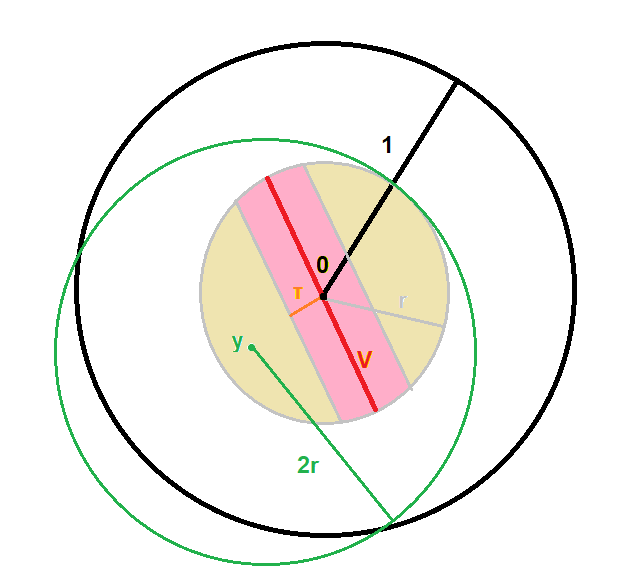
\includegraphics[scale = 0.6]{conesplit}
	\caption{The parameters $\tau \ll r \ll 1$ are chosen as a technical condition such that we have $B_{\tau} (V^k) \cap B_1 (0) \subseteq B_1 (0)$ and $B_r (0) \subseteq B_{2r} (y) \subseteq B_2 (0)$. Cone-splitting occurs in the ball $B_r (0)$.}
\end{center}	
\end{figure}


\begin{corollary}
	Let $f: B_2 (0) \to N^m$ be a stationary harmonic map with bounded energy $E[f] \leq \Lambda$. For every $\eta > 0$ and radii $\tau \ll r \ll 1$, there exists $\epsilon \ll_{n, N, \Lambda, \eta, \tau, r} 1$ such that if there exists $x \in B_r (0)$ such that 
	\begin{enumerate}
		\item $f$ is not $(\eta, r, k + 1)$-homogeneous at $x$, and
		\item $f$ is $(\epsilon, 2r, 0)$-homogeneous at $x$,\label{cor:coneb}
	\end{enumerate}
	then there exists a $k$-plane $V^k \subseteq \R^n$ such that 
		\[ \{ y \in B_r (0) : \text{$f$ is $(\epsilon, 2r, 0)$-homogeneous at $y$} \} \subseteq B_{\tau r} (V^k) .\] \label{cor:cone}
\end{corollary}

\begin{figure}[h]
\begin{center}
	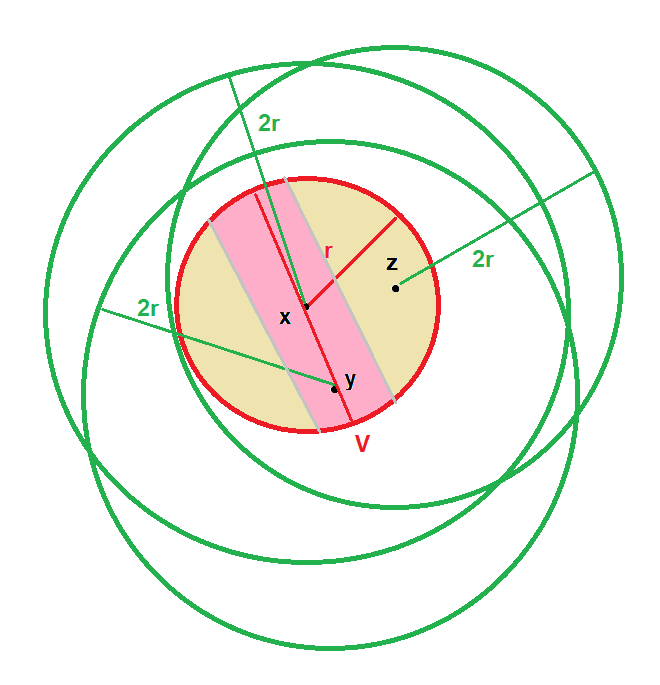
\includegraphics[scale = 0.6]{conesplit2}
	\caption{Sketch of proof for $k = 1$; assume otherwise, then there are $\{x_i\}_i, \{y_i\}_i, \{z_i\}_i$ satisfying (b) where $\{x_i, y_i, z_i\}$ are $\tau$-linearly independent, apply cone-splitting to get contradiction in the limit.}
\end{center}	
\end{figure}
